\graphicspath{ {./hardware/pictures/} }
\section{Hardware}
This section describes which kind of hardware is required and should give an overview about
the used boards. 

\subsection{ESP32-CAM Board}
The ESP32-S-CAM board has different pins and connectors. Additional you will find
a connector panel for the cam, a micro-sd-card-slot, two LED's, a reset button and a connector for an external antenna (this can be not used, because there is a resistance which uses the onboard pcb antenna \cite{YoutubeESP32CamAntenna}).
The table \ref{tab:board-specifications} show you the board specifications.

\begin{table}[H]
\begin{tabular}{lll}
CPU:                     &                                       &                                                    \\ \hline
\multicolumn{1}{l|}{}    & \multicolumn{1}{l|}{Processor:}       & \multicolumn{1}{l|}{Xtensa 32-bit LX6 \cite{ESP32Net}}             \\ \cline{2-3} 
\multicolumn{1}{l|}{}    & \multicolumn{1}{l|}{Cores:}           & \multicolumn{1}{l|}{2}                             \\ \cline{2-3} 
\multicolumn{1}{l|}{}    & \multicolumn{1}{l|}{Clock frequency:} & \multicolumn{1}{l|}{240 MHz \cite{ESP32Net}}                       \\ \cline{2-3} 
\multicolumn{1}{l|}{}    & \multicolumn{1}{l|}{Performance:}     & \multicolumn{1}{l|}{600 DMIPS \cite{ESP32Net}}                     \\ \cline{2-3} 
Memory:                  &                                       &                                                    \\ \hline
\multicolumn{1}{l|}{}    & \multicolumn{1}{l|}{ROM:}             & \multicolumn{1}{l|}{448 KiB \cite{ESP32Net}}                       \\ \cline{2-3} 
\multicolumn{1}{l|}{}    & \multicolumn{1}{l|}{SRAM:}            & \multicolumn{1}{l|}{520 KiB \cite{ESP32Net}}                       \\ \cline{2-3} 
\multicolumn{1}{l|}{}    & \multicolumn{1}{l|}{PSRAM:}           & \multicolumn{1}{l|}{4 MiB \cite{ESP32Net}}                         \\ \cline{2-3} 
Wireless Connectivity:   &                                       &                                                    \\ \hline
\multicolumn{1}{l|}{}    & \multicolumn{1}{l|}{Wi-Fi:}           & \multicolumn{1}{l|}{802.11 b/g/n \cite{ESP32Net}}                  \\ \cline{2-3} 
\multicolumn{1}{l|}{}    & \multicolumn{1}{l|}{Bluetooth:}       & \multicolumn{1}{l|}{v4.2 BR/EDR and BLE Standards \cite{ESP32Net}} \\ \cline{2-3} 
Wi-Fi Security:          & \multicolumn{1}{l|}{}                 & \multicolumn{1}{l|}{WPA/WPA2/WPA2-Enterprise/WPS \cite{LoborisEUESP32CAM}}  \\ \hline
UART Baudrate (default): & \multicolumn{1}{l|}{}                 & \multicolumn{1}{l|}{115200 bps \cite{LoborisEUESP32CAM}}                    \\ \hline
\end{tabular}
\caption{\label{tab:board-specifications}Board specifications}
\end{table}

\begin{figure}[H]
\centering
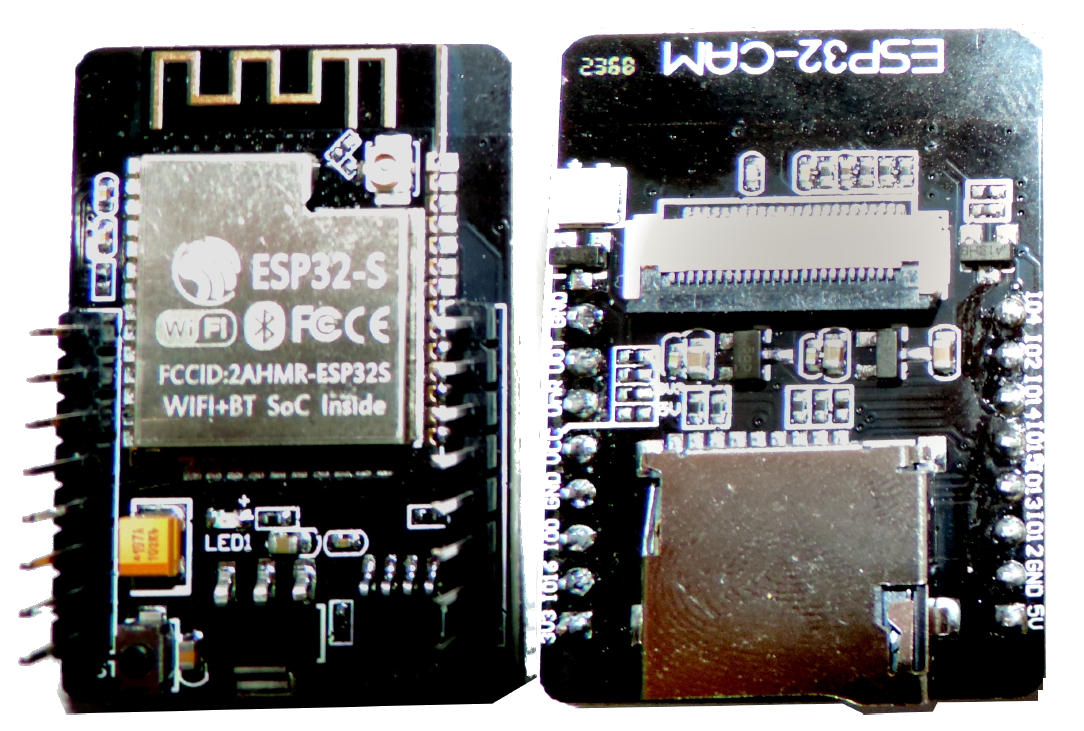
\includegraphics[width=0.75\textwidth]{esp32-s_overview}
\caption[ESP32-S-CAM Overview]{ESP32-S CAM \\ Source: own picture}
\label{ESP32-S-CAM-overview}
\end{figure}

As shown in figure \ref{ESP32-CAM-pinout}, you see the different pinouts of the ESP32-CAM board.

\begin{figure}[H]
\centering
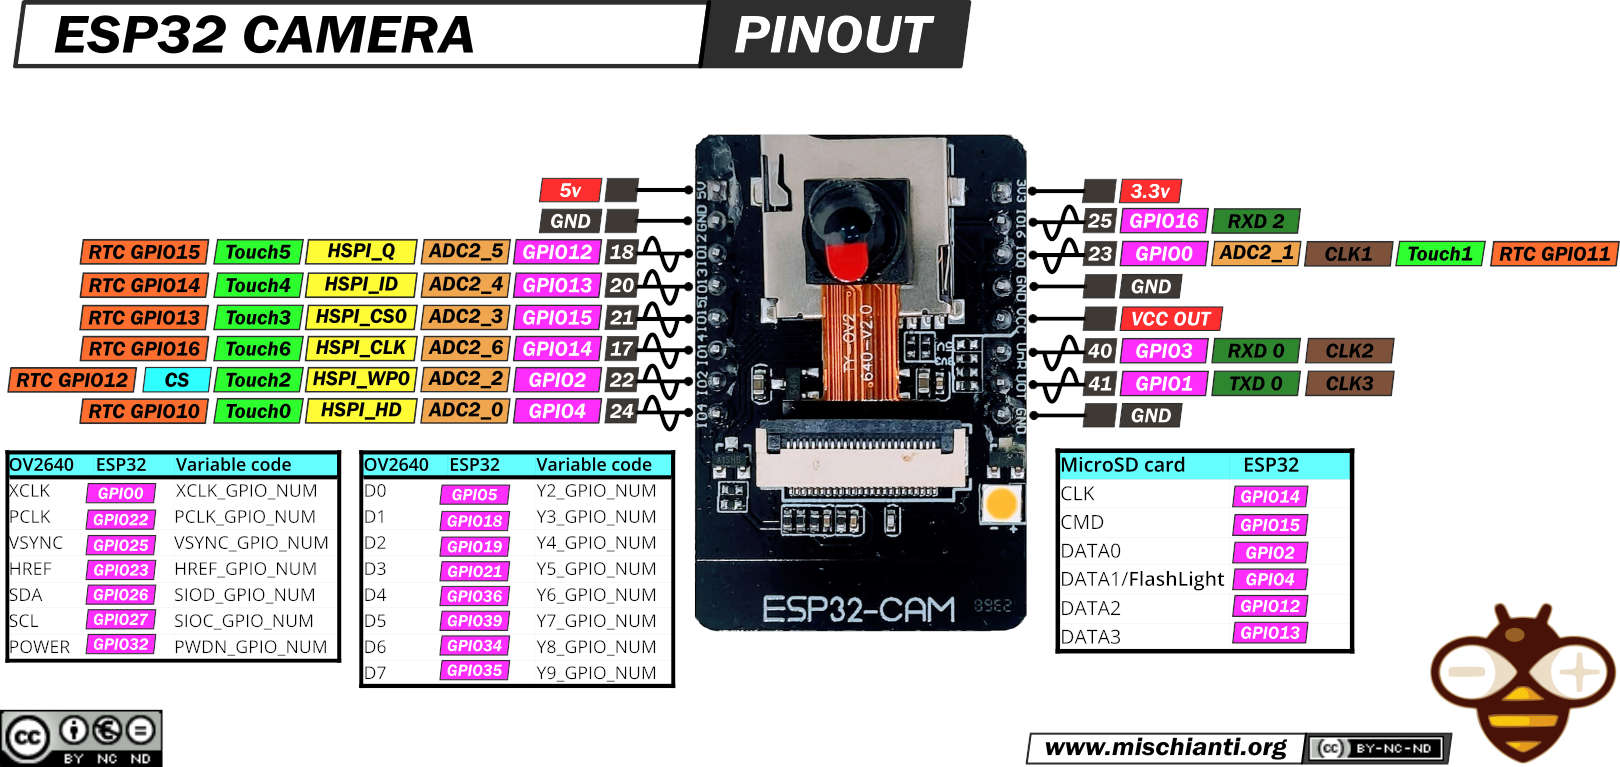
\includegraphics[width=\textwidth]{ESP32-CAM-pinout-mischianti}
\caption[ESP32 CAMERA PINOUT Overview]{ESP32 CAMERA PINOUT \\ Source: \url{https://www.mischianti.org/wp-content/uploads/2020/09/ESP32-CAM-pinout-mischianti.jpg}\\ from Renzo Mischianti \\ License: \url{https://creativecommons.org/licenses/by-nc-nd/4.0/}}
\label{ESP32-CAM-pinout}
\end{figure}

In the picture \ref{ESP32-CAM-backside} you can see the backside of the ESP32-S CAM board. There are the reset-button (in the green box), the internal led (in the blue box) and the (not usable) connector for an external antenna (in the orange box).

\begin{figure}[H]
\centering
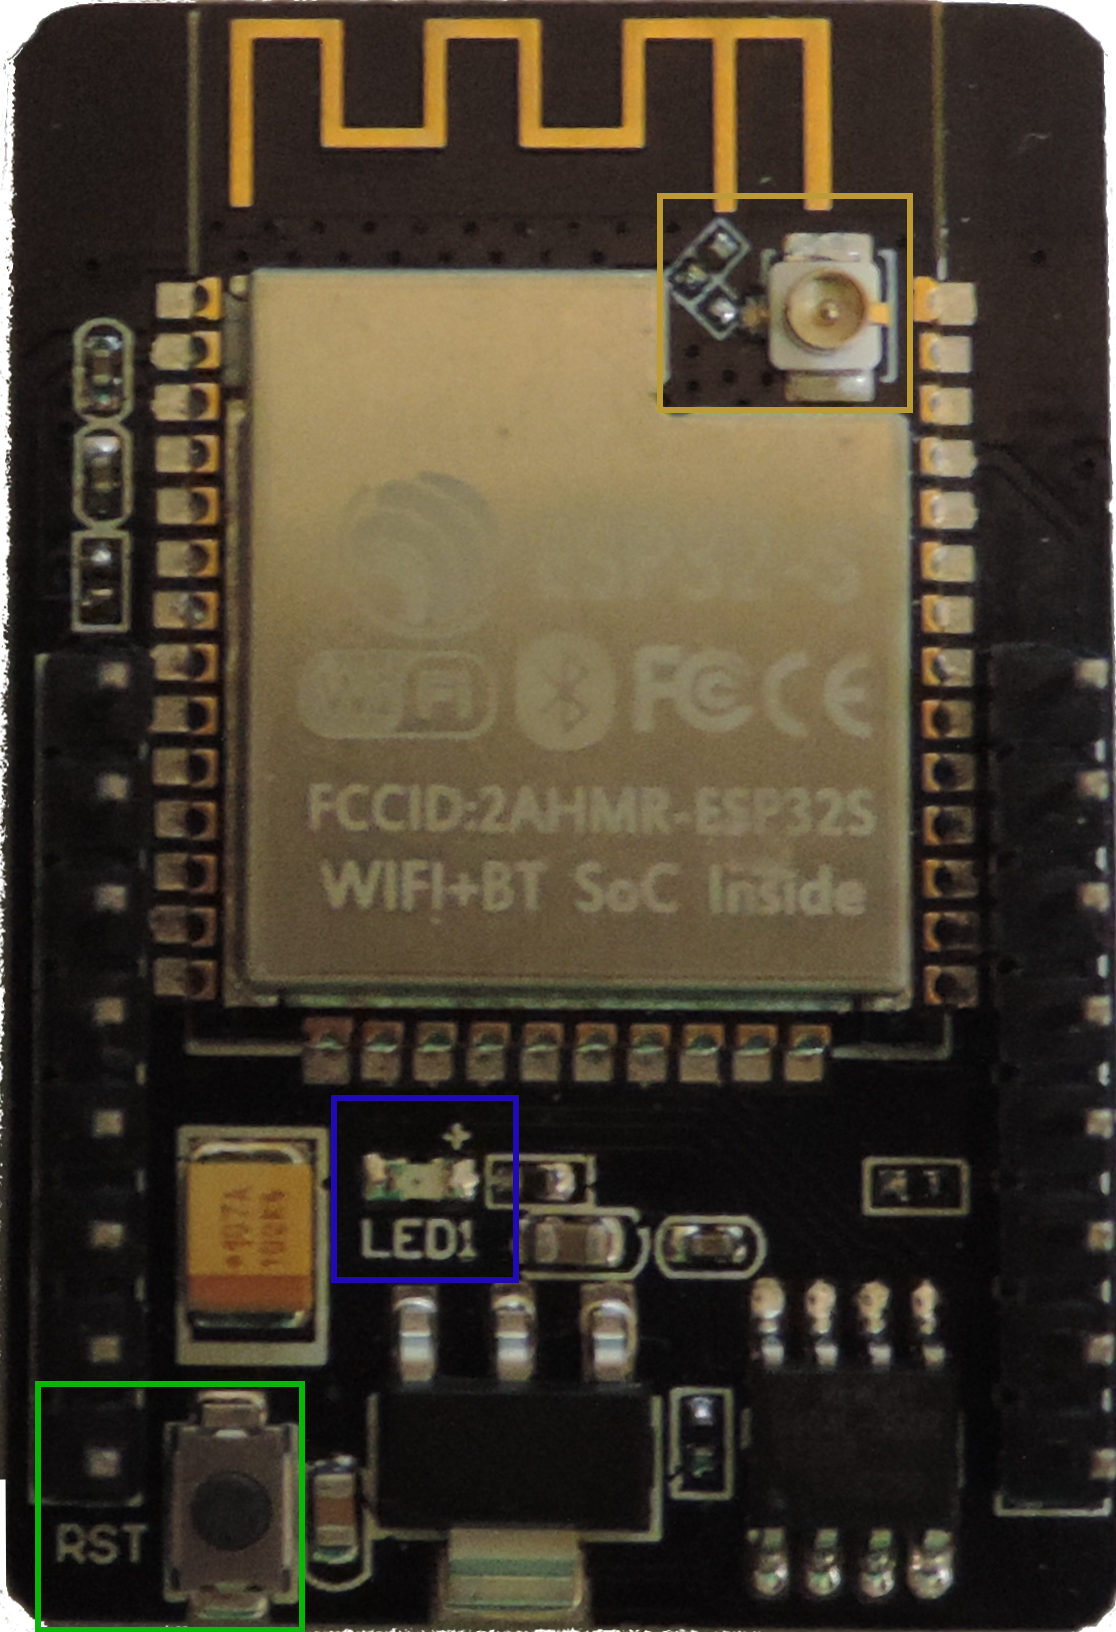
\includegraphics[width=0.75\textwidth]{esp32-s-cam_backside-components}
\caption[ESP32 CAMERA Backside]{ESP32 CAMERA Backside \\ Source: own picture}
\label{ESP32-CAM-backside}
\end{figure}

\subsection{ESP32-CAM MB Programmer Board}
The ESP32-CAM MB Programmer is an optional board. It is a nice to have and with this board it is also possible (as the name already says) to program the ESP32-CAM. In this documentation it will not described how you can programm your ES32-CAM board with the MB programmer board. Additionally the most documentations describes how to upload source-code with the Arduino IDE, which will also not shown in this documentation.

\begin{figure}[H]
\centering
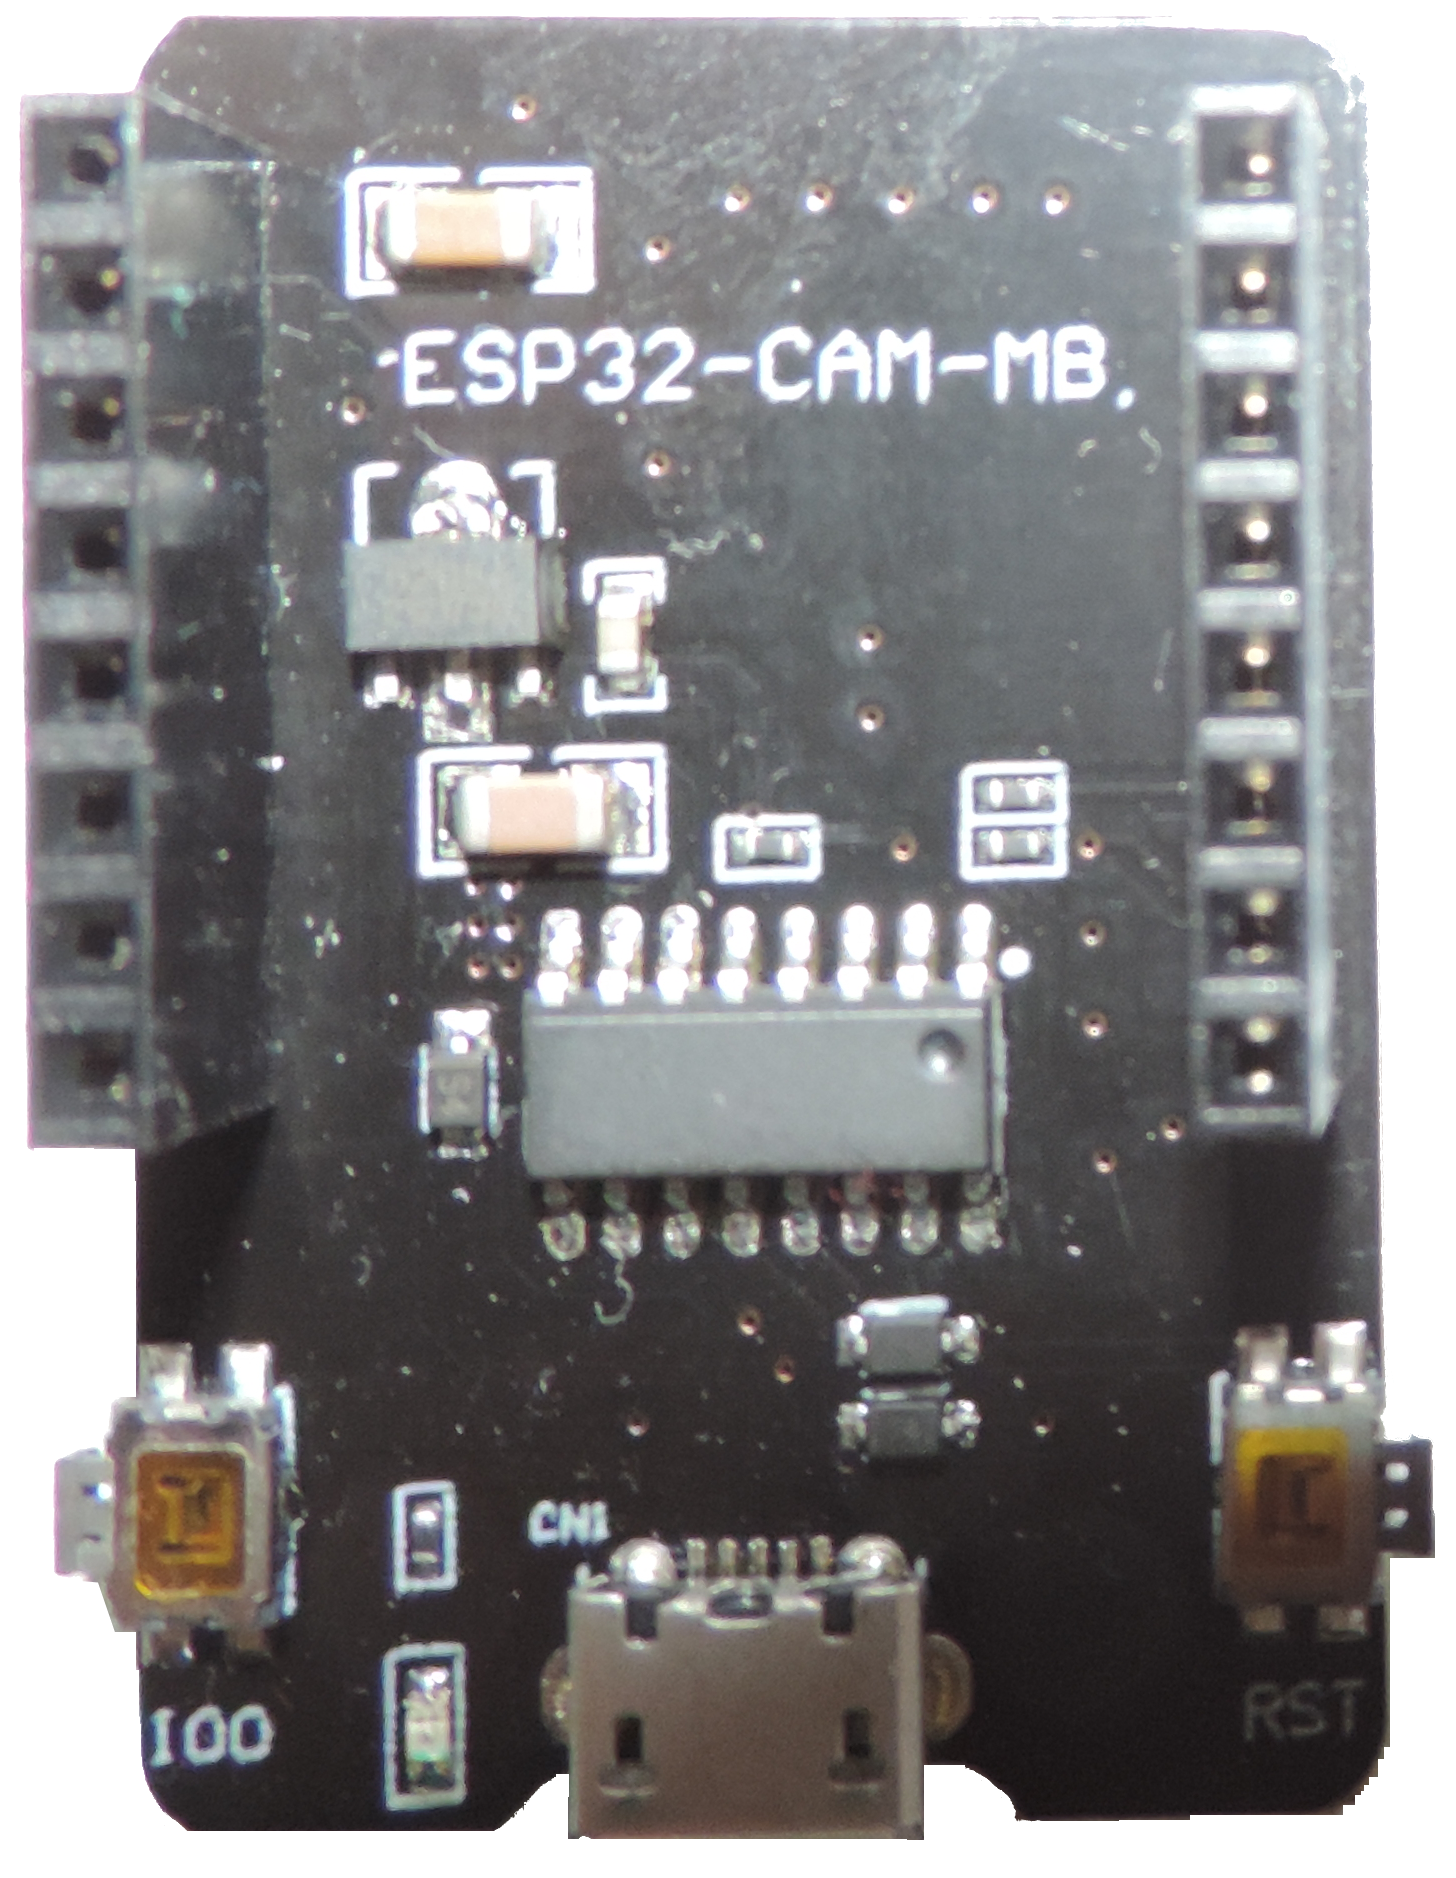
\includegraphics[width=0.4\textwidth]{ESP32-CAM-MB-programmer}
\caption[ESP32-S CAM MB Programmer Board]{ESP32-S CAM MB Programmer Board \\ Source: own picture}
\label{ESP32-S-CAM-overview}
\end{figure}

This board will be used later as power-supply for the ESP32-CAM board.

\subsection{USB to TTL Serial Adapter}
The USB to TTL serial adapter will be used for programming the ESP32-CAM Board.
It is important that it supports 5V, because the ESP32-CAM board needs 5 V input voltage.

\begin{figure}[H]
\centering
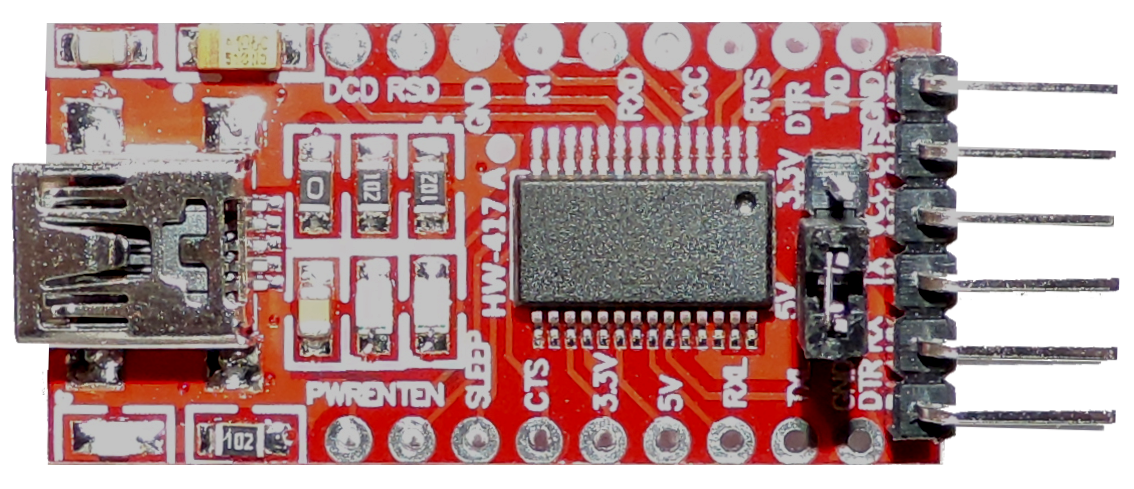
\includegraphics[width=0.7\textwidth]{usb-ttl_serial}
\caption[USB to TTL Serial modul]{USB to TTL Serial modul \\ Source: own picture}
\label{USB-to-TTL-Serial}
\end{figure}

In the picture \ref{USB-to-TTL-Serial} you see a USB to TTL Serial modul that has a Jumper, where you can select the voltage (3 or 5 v). Please put it on the correct slot, that on VCC are 5 V output voltage. 

